\section{\Fv s}
\label{sect:ksfv}

\Fv s are important for shaping the geometrical structure of the global
attractor in a dissipative system.
\Fv s of a pre/relative \po\ stratify the
neighborhood of this orbit. They give a rough picture of the dynamics
close to this orbit. On the other hand,
the stable and unstable manifolds of this orbit are tangent to the \Fv s,
so numerically we grow the unstable manifolds from unstable \Fv s.
Thus, \Fv s provide a way of studying the dynamics far away from this
orbit.
Calculating \Fv s is not an easy task due to the
large range of orders of expansion/contraction rates indicated by
\reftab{tab:floquet_ppo1}. However, with the invention of \ped\ algorithm
(\refchap{chap:ped}), we are able to get a full set of \Fv s at each point of a
pre/relative \po.

\begin{figure}[h]
  \centering
  \begin{minipage}{.47\textwidth}
    \centering \small{\texttt{(a)}}
    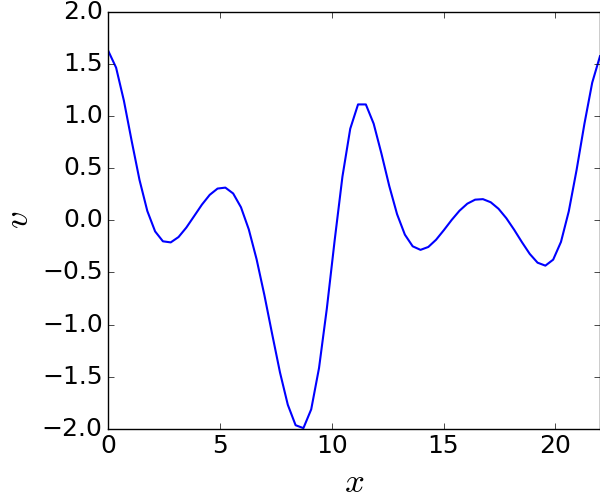
\includegraphics[width=\textwidth]{ksppo1fvt0v1r}
  \end{minipage}
  \begin{minipage}{.47\textwidth}
    \centering \small{\texttt{(b)}}
    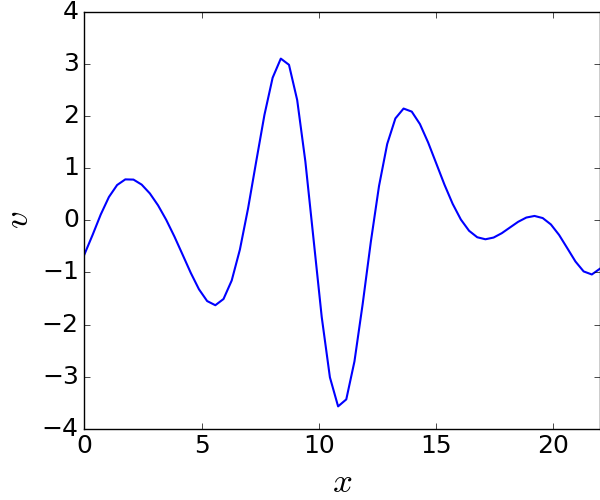
\includegraphics[width=\textwidth]{ksppo1fvt0v5}
  \end{minipage}
  \begin{minipage}{.47\textwidth}
    \centering \small{\texttt{(c)}}
    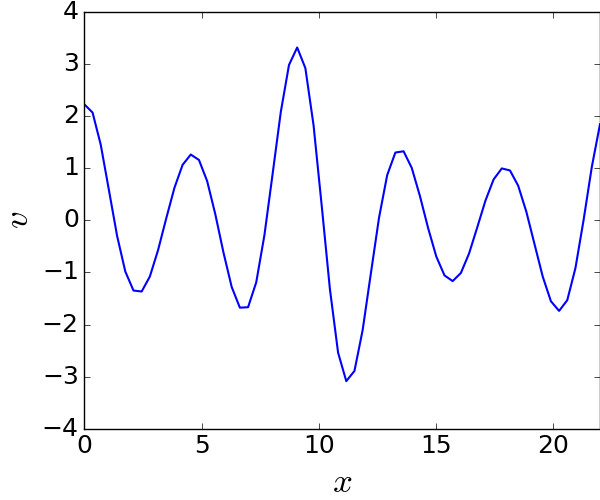
\includegraphics[width=\textwidth]{ksppo1fvt0v10}
  \end{minipage}
  \begin{minipage}{.47\textwidth}
    \centering \small{\texttt{(d)}}
    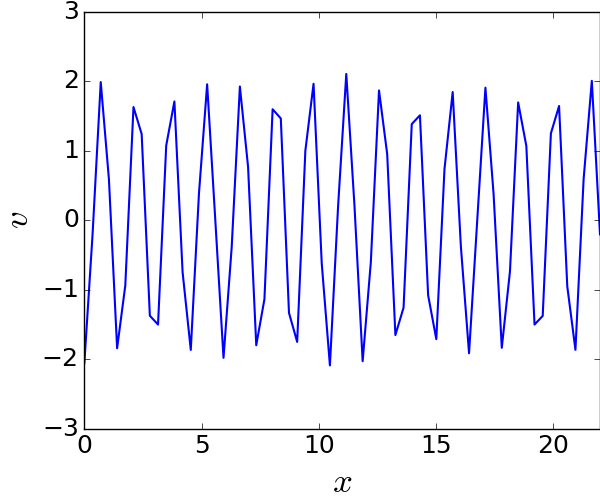
\includegraphics[width=\textwidth]{ksppo1fvt0v30}
  \end{minipage}
  \caption[\Fv s of \PPO{10.25} at $t=0$.]{
    \Fv s of \PPO{10.25} at $t=0$ in \reffig{fig:kspoT100}.
    (a) is the real part of the 1st \Fv.
    (b), (c) and (d) are the $5$th, $10$th, and $30$th \Fv s.
  }
  \label{fig:ksfvt0}
\end{figure}

\begin{figure}[h]
  \centering
  \begin{minipage}{.115\textwidth}
    \centering \small{\texttt{(a)}}
    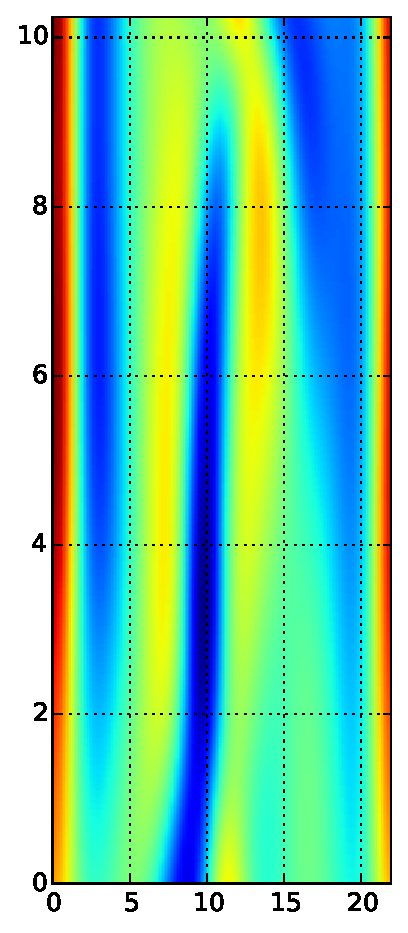
\includegraphics[width=\textwidth]{ppo1Fv1_64}
  \end{minipage}
  \begin{minipage}{.115\textwidth}
    \centering \small{\texttt{(b)}}
    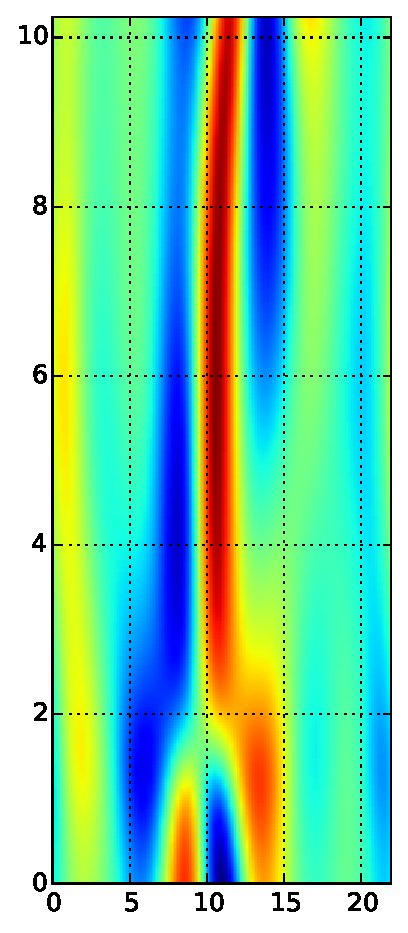
\includegraphics[width=\textwidth]{ppo1Fv5_64}
  \end{minipage}
  \begin{minipage}{.115\textwidth}
    \centering \small{\texttt{(c)}}
    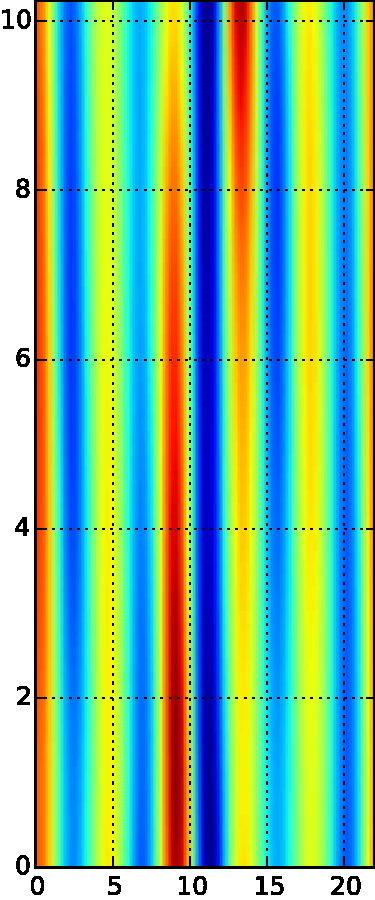
\includegraphics[width=\textwidth]{ppo1Fv10_64}
  \end{minipage}
  \begin{minipage}{.115\textwidth}
    \centering \small{\texttt{(d)}}
    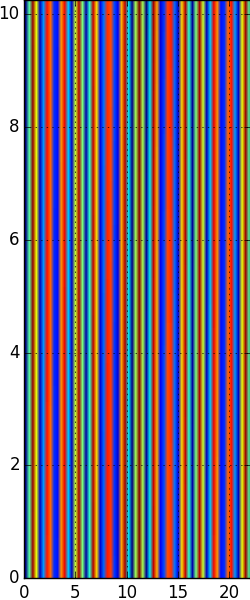
\includegraphics[width=\textwidth]{ppo1Fv30_64}
  \end{minipage}
  \begin{minipage}{.115\textwidth}
    \centering \small{\texttt{(e)}}
    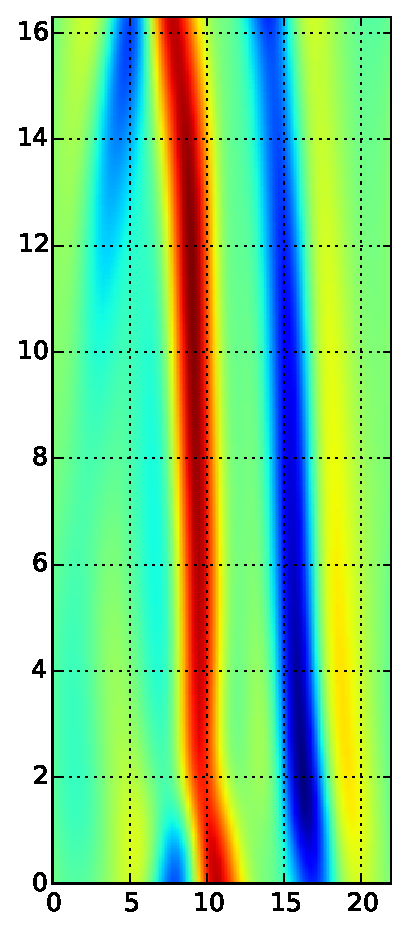
\includegraphics[width=\textwidth]{rpo1Fv1_64}
  \end{minipage}
  \begin{minipage}{.115\textwidth}
    \centering \small{\texttt{(f)}}
    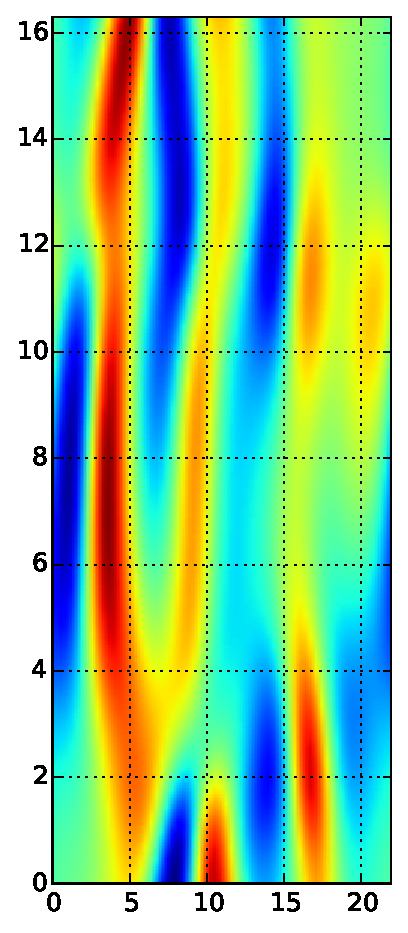
\includegraphics[width=\textwidth]{rpo1Fv4_64}
  \end{minipage}
  \begin{minipage}{.115\textwidth}
    \centering \small{\texttt{(g)}}
    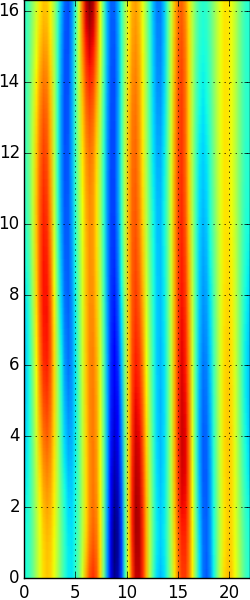
\includegraphics[width=\textwidth]{rpo1Fv10_64}
  \end{minipage}
  \begin{minipage}{.115\textwidth}
    \centering \small{\texttt{(h)}}
    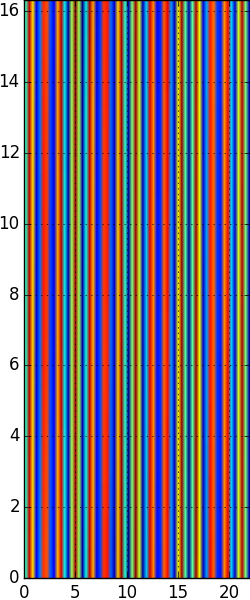
\includegraphics[width=\textwidth]{rpo1Fv30_64}
  \end{minipage}%
  \caption[\Fv s of \PPO{10.25} and \RPO{16.31} for one prime period.]{
    (a) $\sim$ (d) : the 1st (real part), 5th, 10th and 30th \Fv\ along
    \PPO{10.25} for one prime period.
    (e) $\sim$ (h) : the 1st, 4th (real part), 10th (imaginary part) 30th (imaginary part)
    \Fv\ along \RPO{16.31} for one prime period.
    Axes and color scale are the same as \reffig{fig:kspoT100}.
  }
  \label{fig:Fvs}
\end{figure}
\begin{figure}[h]
  \centering
  \begin{minipage}{.47\textwidth}
    \centering \small{\texttt{(a)}}
    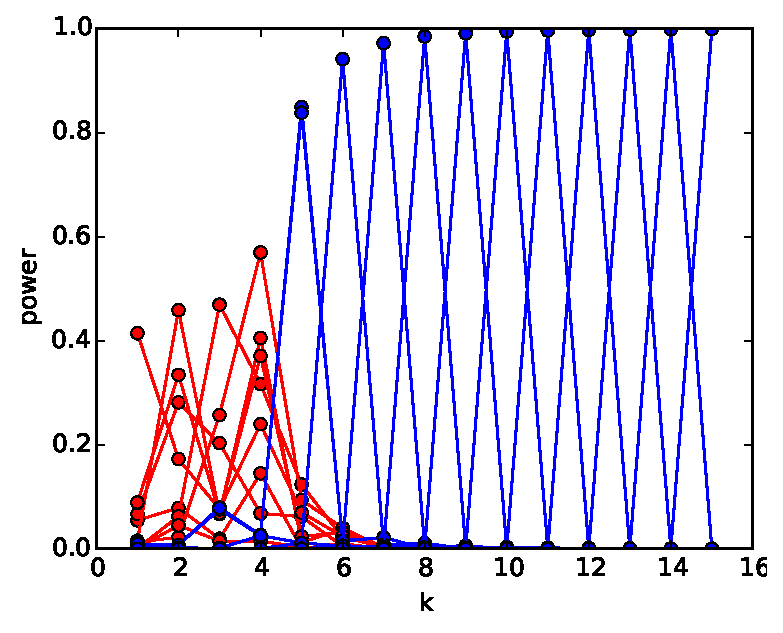
\includegraphics[width=\textwidth]{ppo1power64}
  \end{minipage}
  \begin{minipage}{.47\textwidth}
    \centering \small{\texttt{(b)}}
    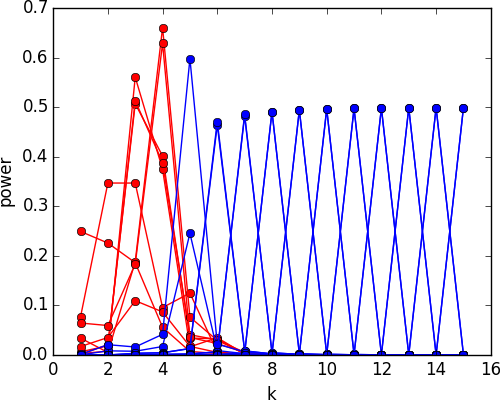
\includegraphics[width=\textwidth]{rpo1power64}
  \end{minipage}
  \caption[The power spectrum of the first 30 \Fv s for \PPO{10.25} and \RPO{16.31}.]{
    The power spectrum of the first 30 \Fv s for \PPO{10.25}
    (left) and \RPO{16.31} (right)
    at $t=0$. Red lines correspond to the leading 8 \Fv s; while
    the blue lines correspond to the left 22 \Fv s with the $i${th} one
    localized at index $\lceil \frac{i}{2} \rceil$.
    Power at index $k$ is defined to be the square of the $k_{th}$
    Fourier coefficient's magnitude
    of \Fv s.
    The $x$-axis is
    labeled by the Fourier mode indices.
    Only the $k>0$ part is shown, and the part for
    negative $k$ follows by reflection. For complex \Fv s, the
    power spectra of the real part and imaginary part are calculated
    separately. Since almost all contracting \Fv s of \RPO{16.31}
    form complex conjugate pairs, their power peaks are far less than 1,
    as shown in panel (b).
  }
  \label{fig:FVpower}
\end{figure}

\refFig{fig:ksfvt0} shows the real part of the 1st \Fv, the 5th,
the 10th and 30th \Fv s of \PPO{10.25}. As index increases, \Fv s behave more
like pure Fourier modes.
\refFig{fig:Fvs} shows a few selected \Fv s along \PPO{10.25}
and \RPO{16.13} for one prime period respectively.
We can see that the \spt\ plots of the few leading
Fv s, see panels (a,b) and (e,f), exhibit turbulent structures containing only long waves,
for both \PPO{10.25} and \RPO{16.13},
but for
\Fv s corresponding to strong contraction rates, \ie, panels (c,d), (g,h),
the configurations
are almost pure sinusoidal curves. The power spectra in \refFig{fig:FVpower}
demonstrate this point too. The leading 8 \Fv s have large components in
the first 5 Fourier modes and the spectra are entangled with each other;
while the remaining \Fv s almost concentrate
on a single Fourier mode and are decoupled from each other;
more specifically, the $i$th \Fv\ with $i\ge 9$
peaks at the $\lceil \frac{i}{2} \rceil$th\footnote{{
Here, $\lceil x \rceil$ denotes the smallest integer no less than $x$. }}
mode in \reffig{fig:FVpower}.
Takeuchi {\etal}\rf{TaGiCh11, YaTaGiChRa08} observe similar
features in \cLv s along ergodic
trajectories and by measuring the tangency between these two groups of
\cLv s, they reach a reasonable conclusion about the dimension of
the inertial manifold in \KSe\ and \cGLe.
Therefore, we anticipate that analyzing the tangency of \Fv s along
different pre/relative \po s can also lead to the same conclusion, which
will be discussed in detail in \refchap{chap:im}.
